% Options for packages loaded elsewhere
\PassOptionsToPackage{unicode}{hyperref}
\PassOptionsToPackage{hyphens}{url}
%
\documentclass[
  11pt,
]{article}
\usepackage{amsmath,amssymb}
\usepackage{iftex}
\ifPDFTeX
  \usepackage[T1]{fontenc}
  \usepackage[utf8]{inputenc}
  \usepackage{textcomp} % provide euro and other symbols
\else % if luatex or xetex
  \usepackage{unicode-math} % this also loads fontspec
  \defaultfontfeatures{Scale=MatchLowercase}
  \defaultfontfeatures[\rmfamily]{Ligatures=TeX,Scale=1}
\fi
\usepackage{lmodern}
\ifPDFTeX\else
  % xetex/luatex font selection
  \setmainfont[]{Times New Roman}
\fi
% Use upquote if available, for straight quotes in verbatim environments
\IfFileExists{upquote.sty}{\usepackage{upquote}}{}
\IfFileExists{microtype.sty}{% use microtype if available
  \usepackage[]{microtype}
  \UseMicrotypeSet[protrusion]{basicmath} % disable protrusion for tt fonts
}{}
\makeatletter
\@ifundefined{KOMAClassName}{% if non-KOMA class
  \IfFileExists{parskip.sty}{%
    \usepackage{parskip}
  }{% else
    \setlength{\parindent}{0pt}
    \setlength{\parskip}{6pt plus 2pt minus 1pt}}
}{% if KOMA class
  \KOMAoptions{parskip=half}}
\makeatother
\usepackage{xcolor}
\usepackage[margin=1in]{geometry}
\usepackage{graphicx}
\makeatletter
\def\maxwidth{\ifdim\Gin@nat@width>\linewidth\linewidth\else\Gin@nat@width\fi}
\def\maxheight{\ifdim\Gin@nat@height>\textheight\textheight\else\Gin@nat@height\fi}
\makeatother
% Scale images if necessary, so that they will not overflow the page
% margins by default, and it is still possible to overwrite the defaults
% using explicit options in \includegraphics[width, height, ...]{}
\setkeys{Gin}{width=\maxwidth,height=\maxheight,keepaspectratio}
% Set default figure placement to htbp
\makeatletter
\def\fps@figure{htbp}
\makeatother
\setlength{\emergencystretch}{3em} % prevent overfull lines
\providecommand{\tightlist}{%
  \setlength{\itemsep}{0pt}\setlength{\parskip}{0pt}}
\setcounter{secnumdepth}{-\maxdimen} % remove section numbering
\usepackage{setspace}
\doublespacing
\usepackage{booktabs}
\usepackage{longtable}
\usepackage{array}
\usepackage{multirow}
\usepackage{wrapfig}
\usepackage{float}
\usepackage{colortbl}
\usepackage{pdflscape}
\usepackage{tabu}
\usepackage{threeparttable}
\usepackage{threeparttablex}
\usepackage[normalem]{ulem}
\usepackage{makecell}
\usepackage{xcolor}
\ifLuaTeX
  \usepackage{selnolig}  % disable illegal ligatures
\fi
\IfFileExists{bookmark.sty}{\usepackage{bookmark}}{\usepackage{hyperref}}
\IfFileExists{xurl.sty}{\usepackage{xurl}}{} % add URL line breaks if available
\urlstyle{same}
\hypersetup{
  pdftitle={71point4 Analyst Assignment},
  pdfauthor={André le Roux},
  hidelinks,
  pdfcreator={LaTeX via pandoc}}

\title{71point4 Analyst Assignment}
\author{André le Roux}
\date{2024-08-21}

\begin{document}
\maketitle

\hypertarget{question-3}{%
\section{Question 3}\label{question-3}}

I was unsure of the level of difficulty that the question should be, so
I decided to go for a question with two parts that can be given
individually or together.

\hypertarget{part-a}{%
\subparagraph{Part A:}\label{part-a}}

You are a supplier of wood and own a 20km by 10km forest on which you
plant trees. Assume that the trees are equally distributed and that the
number of trees tends to infinity. As you want to monitor the forest you
set up 158 microphones that each monitor a 1km by 1km area.

What is the probability of hearing at least one of every 2 trees that
fall in the forest sequentially?

\hypertarget{part-b}{%
\subparagraph{Part B:}\label{part-b}}

There exits a 4 digit number x, where each digit consists of a unique
number. The number x has the following characteristics:

\begin{itemize}
\tightlist
\item
  The first two digits of x form a prime number.
\item
  the second two digits are a square.
\item
  x - 1 is also a prime number.
\item
  It is divisible by the nearest rounded percentage of part A.
\end{itemize}

What number is x?

\hypertarget{question-4}{%
\section{Question 4}\label{question-4}}

\hypertarget{graph-4.1}{%
\subsection{Graph 4.1}\label{graph-4.1}}

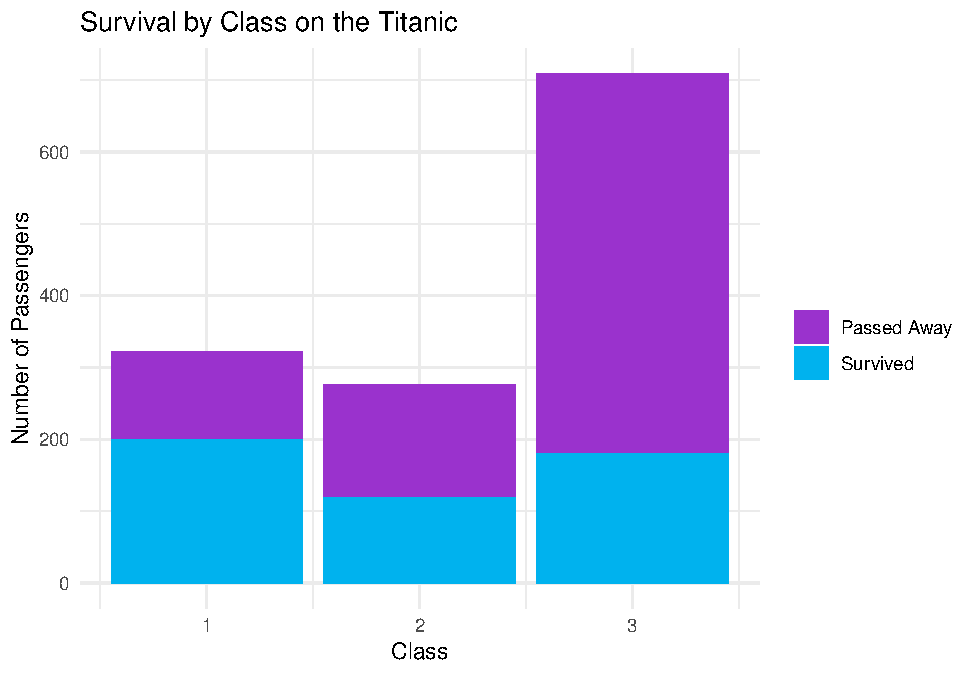
\includegraphics{README_files/figure-latex/unnamed-chunk-2-1.pdf}

This first graph gives us a visual representation of the number of
surviving passengers in different classes. As can be seen the chances of
surviving is lowest for passengers in the lowest class (third), at
slightly above 25\%. While the passengers in first class had an
approximately 62.5\% chance of survival. It should also be noted that
the number of passengers in the third class significantly outweigh the
number of passengers in the first and second class.

\hypertarget{graph-4.2}{%
\subsection{Graph 4.2}\label{graph-4.2}}

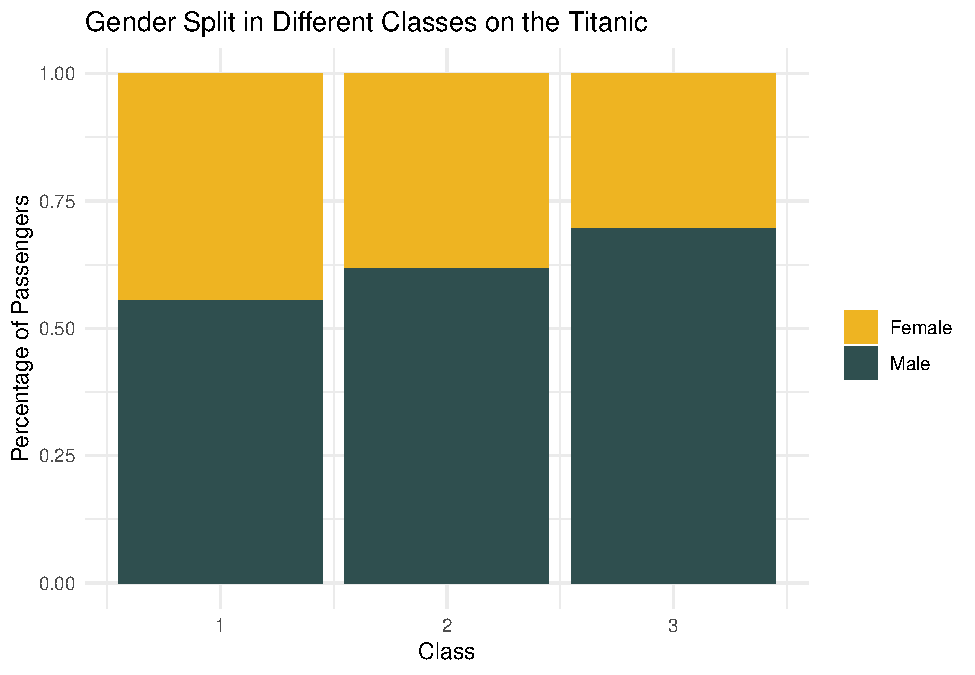
\includegraphics{README_files/figure-latex/unnamed-chunk-3-1.pdf}

It is noticeable from this graph that the percentage of men differ
between classes. With the composition becoming more male orientated the
lower the class. In the first class it is only slightly male orientated,
with 55.42\% of the passengers being male. However, in the third class
the male percentage rises to 69.53\% of the passengers.

\hypertarget{graph-4.3}{%
\subsection{Graph 4.3}\label{graph-4.3}}

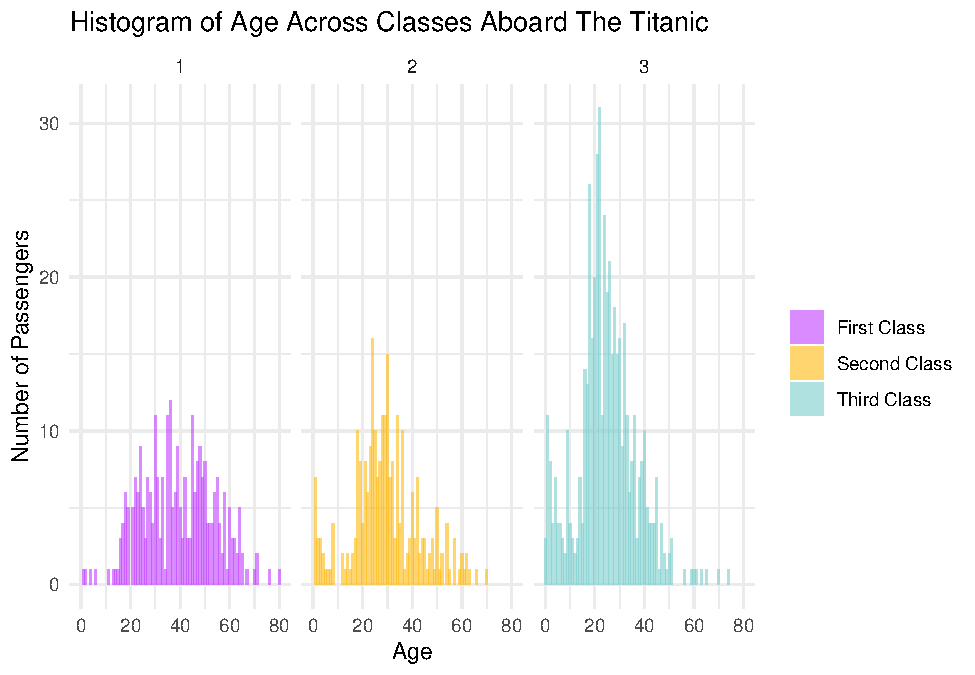
\includegraphics{README_files/figure-latex/unnamed-chunk-4-1.pdf}

Here we can see a side by side comparisons of the age compositions of
the different classes aboard the Titanic. From this comparison we can
see that the third class was composed of a higher percentage of younger
people than first or second class. With first class being the least
skewed of the three classes.

\hypertarget{graph-4.4}{%
\subsection{Graph 4.4}\label{graph-4.4}}

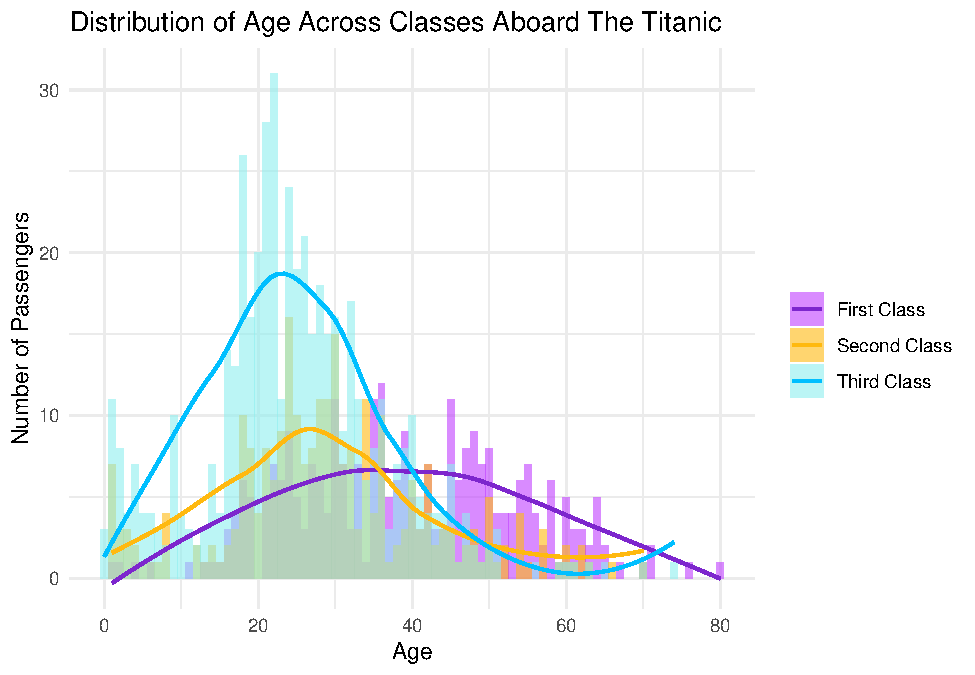
\includegraphics{README_files/figure-latex/unnamed-chunk-5-1.pdf}

In this graph we overlap the histogram plots and add a smoothed line to
represent the possible underlying distribution. By overlapping the plots
we can easily compare the various distributions, from this we can see
that the age of third class passengers is more right skewed than the
other classes. The first class on the other hand, has a skewness value
closer to 0.

\hypertarget{graph-4.5}{%
\subsection{Graph 4.5}\label{graph-4.5}}

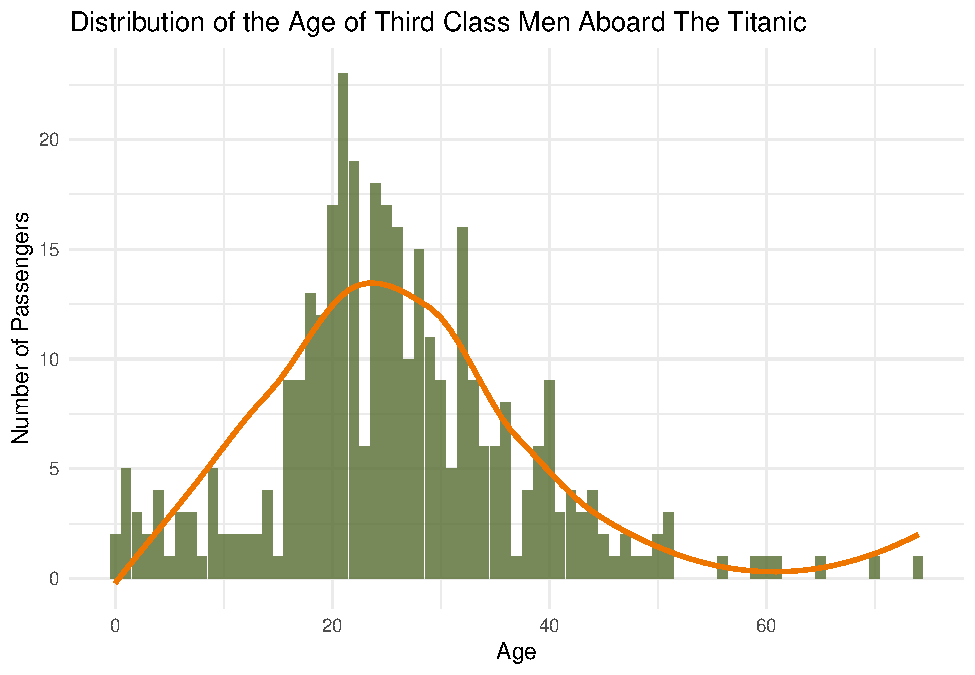
\includegraphics{README_files/figure-latex/unnamed-chunk-6-1.pdf}

We can see from this plot that the men in the third class on-board the
titanic was mostly younger men from their teens to early thirties, with
the mode age being 21. This suggests that they were passengers that were
willing to forego a certain degree of comfort in order to be part of the
first journey of the Titanic and to reach America. These are people that
might not have been able to afford more expensive means of travel, but
wanted to start a new life in America.

\hypertarget{graph-4.6}{%
\subsection{Graph 4.6}\label{graph-4.6}}

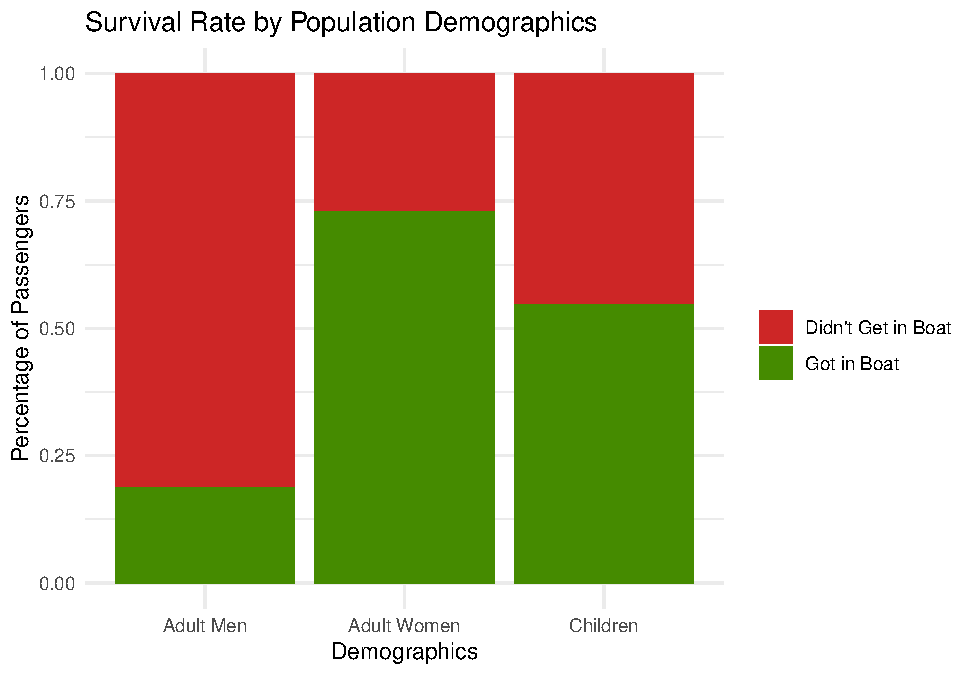
\includegraphics{README_files/figure-latex/unnamed-chunk-7-1.pdf}

From this graph it becomes clear that women and children had priority
when getting onto lifeboats. Less than 20\% of adult men got into
lifeboats, while more than 70\% of adult women got into lifeboats. It
should also be noted that barely more than 50\% of children got into
lifeboats. This might suggest that preferences might have also fallen
along class lines with children from the second and third classes having
a lower probability of getting into the lifeboats. This difference in
class would also influence the percentage of passengers in the lifeboats
as third and second class passenger classes consisted of more men.

\hypertarget{bonus-question}{%
\section{Bonus Question}\label{bonus-question}}

In order to predict the probability that a passenger survives the
Titanic shipwreck, based on prior information, I use a Logistic model
that is trained on 80\% of the data with 10-fold cross validation. This
prediction model is then tested on 20\% of the data. The ``caret''
package in R was used to train and test this model. The data used to
train this model consisted of the survived variable as the dependent
variable and age, class, sex, fare, sibsp (number of siblings and
spouses) and parch (number of parents/children on board). Whether they
got into a lifeboat is not included, as a model with this variable
included gives an accuracy of 98.56\% due to the importance of being in
a lifeboat. Thus, we believe a forward looking model from the point of
departure is more interesting.

Although not very aesthetic, I have included a breakdown of the
performance of the model on test data, followed by a variable importance
plot, which states the most and least important variables in predicting
which passengers pass away and which do not.

\begin{verbatim}
## Confusion Matrix and Statistics
## 
##           Reference
## Prediction   0   1
##          0 104  21
##          1  24  60
##                                           
##                Accuracy : 0.7847          
##                  95% CI : (0.7227, 0.8384)
##     No Information Rate : 0.6124          
##     P-Value [Acc > NIR] : 7.94e-08        
##                                           
##                   Kappa : 0.5495          
##                                           
##  Mcnemar's Test P-Value : 0.7656          
##                                           
##             Sensitivity : 0.8125          
##             Specificity : 0.7407          
##          Pos Pred Value : 0.8320          
##          Neg Pred Value : 0.7143          
##              Prevalence : 0.6124          
##          Detection Rate : 0.4976          
##    Detection Prevalence : 0.5981          
##       Balanced Accuracy : 0.7766          
##                                           
##        'Positive' Class : 0               
## 
\end{verbatim}

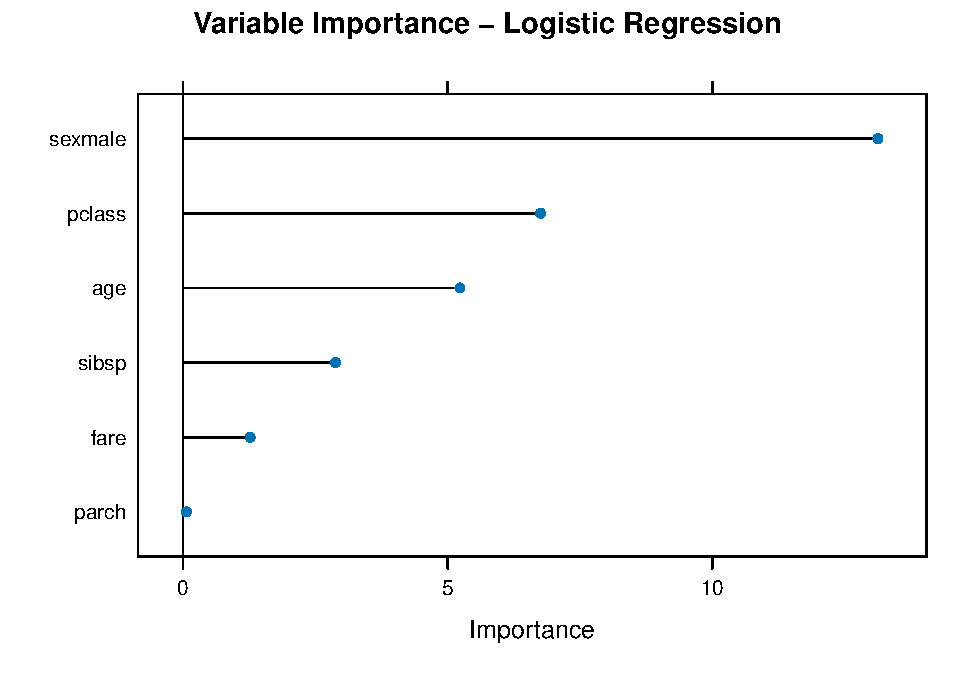
\includegraphics{README_files/figure-latex/unnamed-chunk-8-1.pdf}

This model predicts with an accuracy of 78.47\% and finds that the most
important predictors of survival are sex, which class they are in and
their age. Linearity is not one of the features of a Logistic
regression, for that reason the model can predict the probability given
a vector of specific inputs, but the coefficients are not as easy to
interpret. The coefficients are however still reliable in predicting the
correct direction. From this we can see that the person who is most
likely to survive is a newborn woman in first class, with no siblings
and who had an extremely high fare (550).

Using this model we can also predict individual probabilities. For
example, Rose from the movie Titanic (Woman, 1st class, 17, 0 siblings,
500 fare, 1 parent) would have a 98.62\% chance of survival based on
this model. While Jack Dawson (Man, 3rd class, 20, 0 siblings, 0 fare, 0
parents) only has a 15.54\% chance of survival based on this model.

Thank you for the opportunity to do this project and I hope to hear more
about this interesting opportunity.

\end{document}
